\documentclass[12pt, a4paper]{article}  

\usepackage{etex} % расширение классического tex в частности позволяет подгружать гораздо больше пакетов, чем мы и займёмся далее

%%%%%%%%%% Математика %%%%%%%%%%
\usepackage{amsmath,amsfonts,amssymb,amsthm,mathtools} 
%\mathtoolsset{showonlyrefs=true}  % Показывать номера только у тех формул, на которые есть \eqref{} в тексте.
%\usepackage{leqno} % Нумерация формул слева


%%%%%%%%%%%%%%%%%%%%%%%% Шрифты %%%%%%%%%%%%%%%%%%%%%%%%%%%%%%%%%
\usepackage{fontspec}         % пакет для подгрузки шрифтов
\setmainfont{Arial}   % задаёт основной шрифт документа

\defaultfontfeatures{Mapping=tex-text}

% why do we need \newfontfamily:
% http://tex.stackexchange.com/questions/91507/
\newfontfamily{\cyrillicfonttt}{Arial}
\newfontfamily{\cyrillicfont}{Arial}
\newfontfamily{\cyrillicfontsf}{Arial}

\usepackage{unicode-math}     % пакет для установки математического шрифта
\setmathfont{Asana Math}      % шрифт для математики

\usepackage{polyglossia}      % Пакет, который позволяет подгружать русские буквы
\setdefaultlanguage{russian}  % Основной язык документа
\setotherlanguage{english}    % Второстепенный язык документа


%%%%%%%%%% Работа с картинками %%%%%%%%%
\usepackage{graphicx}                  % Для вставки рисунков
\usepackage{graphics} 
\graphicspath{{images/}{pictures/}}    % можно указать папки с картинками
\usepackage{wrapfig}                   % Обтекание рисунков и таблиц текстом
\usepackage{subfigure}                 % для создания нескольких рисунков внутри одного


%%%%%%%%%% Работа с таблицами %%%%%%%%%%
\usepackage{tabularx}            % новые типы колонок
\usepackage{tabulary}            % и ещё новые типы колонок
\usepackage{array}               % Дополнительная работа с таблицами
\usepackage{longtable}           % Длинные таблицы
\usepackage{multirow}            % Слияние строк в таблице
\usepackage{float}               % возможность позиционировать объекты в нужном месте 
\usepackage{booktabs}            % таблицы как в книгах!  
\renewcommand{\arraystretch}{1.3} % больше расстояние между строками



\usepackage{tikz}  % Пакет для графики. Будем разбирать его на следующей паре.
\usepackage{pgfplots}   % Аналогично  
\usetikzlibrary{arrows}
\usepackage{color}
\usepackage{xcolor}
\usepackage{lscape}
\usepackage{makecell}

\usepackage[margin=15mm]{geometry}
\usepackage{tikz}
\usetikzlibrary{shadows}

\newcommand{\button}[1]%
{   \begin{tikzpicture}[baseline=(tempname.base)]
	\node[draw=red, fill=green, rounded corners=1.5pt, inner sep=2pt, minimum width=1.5em, minimum height=1.2em] (tempname) {#1};
	\end{tikzpicture}
}

\begin{document}
	
 \begin{tabular}{ |c c c c c| }
  \hline
  \multicolumn{5}{|c|}{Питер: туда и обратно 17-19 марта} \\
  \hline
  \textbf{Перевозчик} & \textbf{Москва} & \textbf{Длительность} & \textbf{СПБ} & \textbf{Цена} \\
  \hline
  Ural airlines & \makecell {9:50 \\ \\ 21:40} & 
  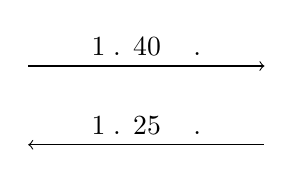
\begin{tikzpicture} 
  \draw [->] (0,1) -- (3,1);
  \draw [<-] (0,0) -- (3,0);
  \node [above] at (1.5,1) {1ч. 40 мин.};
  \node [above] at (1.5,0) {1ч. 25 мин.};
  \end{tikzpicture} 
   & \makecell{11:30 \\ \\ 20:15}  & \makecell{ \huge {2824} \\  \large{\button{Купить}}}	\\
  \hline
  Nordwind airlines& \makecell{7:05 \\ \\ 10:45} &
  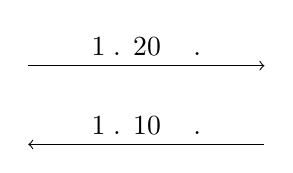
\begin{tikzpicture} 
  \draw [->] (0,1) -- (3,1);
  \draw [<-] (0,0) -- (3,0);
  \node [above] at (1.5,1) {1ч. 20 мин.};
  \node [above] at (1.5,0) {1ч. 10 мин.};
  \end{tikzpicture} 
   & \makecell{8:25 \\ \\ 9:35} & \makecell{ \huge{2958} \\ \large{\button{Купить}}} \\
   \hline
   UTair& \makecell{0:50 \\ \\ 9:40} &
  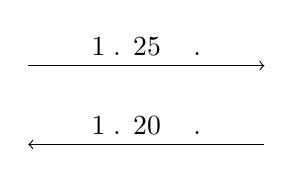
\begin{tikzpicture} 
  \draw [->] (0,1) -- (3,1);
  \draw [<-] (0,0) -- (3,0);
  \node [above] at (1.5,1) {1ч. 25 мин.};
  \node [above] at (1.5,0) {1ч. 20 мин.};
  \end{tikzpicture} 
   & \makecell{2:15\\ \\ 8:20} & \makecell{\huge{2980} \\ \large{\button{Купить}}} \\
  \hline	
    UTair& \makecell{9:25 \\ \\ 8:25} &
  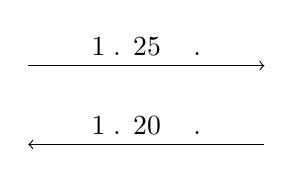
\begin{tikzpicture} 
  \draw [->] (0,1) -- (3,1);
  \draw [<-] (0,0) -- (3,0);
  \node [above] at (1.5,1) {1ч. 25 мин.};
  \node [above] at (1.5,0) {1ч. 20 мин.};
  \end{tikzpicture} 
  & \makecell{10:50 \\ \\ 7:00} & \makecell{ \huge{2980} \\ \large{\button{Купить}}} \\
  \hline
   Сапсан & \makecell{19:40 \\ \\ 14:50} &
  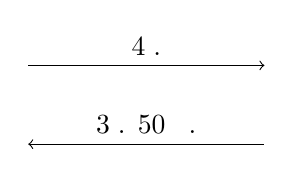
\begin{tikzpicture} 
  \draw [->] (0,1) -- (3,1);
  \draw [<-] (0,0) -- (3,0);
  \node [above] at (1.5,1) {4ч.};
  \node [above] at (1.5,0) {3ч. 50мин.};
  \end{tikzpicture} 
  & \makecell {23:40 \\ \\ 11:00} & \makecell{ \huge{5321} \\ \large{\button{Купить}}} \\
  \hline
   Двухэтажный & \makecell{22:50 \\ \\ 6:45} &
  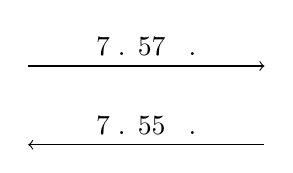
\begin{tikzpicture} 
  \draw [->] (0,1) -- (3,1);
  \draw [<-] (0,0) -- (3,0);
  \node [above] at (1.5,1) {7ч. 57мин.};
  \node [above] at (1.5,0) {7ч. 55мин.};
  \end{tikzpicture} 
  & \makecell{6:47 \\ \\ 22:50} & \makecell{ \huge{3118} \\ \large{\button{Купить}}} \\
  \hline
  Экспресс & \makecell{23:30 \\ \\ 8:30} &
  \begin{tikzpicture} 
  \draw [->] (0,1) -- (3,1);
  \draw [<-] (0,0) -- (3,0);
  \node [above] at (1.5,1) {9ч.};
  \node [above] at (1.5,0) {9ч.};
  \end{tikzpicture} 
  & \makecell{8:30 \\ \\ 23:30} & \makecell{ \huge{4646} \\ \large{\button{Купить}}} \\
  \hline
  Гранд Экспресс & \makecell{23:40 \\ \\ 8:14} &
  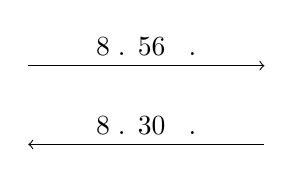
\begin{tikzpicture} 
  \draw [->] (0,1) -- (3,1);
  \draw [<-] (0,0) -- (3,0);
  \node [above] at (1.5,1) {8ч. 56мин.};
  \node [above] at (1.5,0) {8ч. 30мин.};
  \end{tikzpicture} 
  & \makecell{8:36 \\ \\ 23:44} & \makecell{ \huge{8456} \\ \large{\button{Купить}}} \\
  \hline
  	
 \end{tabular}
		
\end{document}
